
\begin{frame}
\frametitle{Identificación de Riesgos}

\begin{itemize}
    \item Identificar los riesgos que puedan afectar el proyecto, documentando
    sus \textbf{características}.
    \item Es un proceso \textbf{iterativo}, ya que nuevos riesgos pueden evolucionar o aparecer en el transcurso del proyecto.
    \item El proceso debe involucrar al los miembros del proyecto para
    inculcar un sentido de \textbf{responsabilidad} en ellos.
\end{itemize}
\begin{columns}
	\begin{column}{0.6\textwidth}
	\end{column}
	\begin{column}{0.4\textwidth}
		\includegraphics[width=3cm]{img/random_img_2}
	\end{column}
\end{columns}
\end{frame}

\begin{frame}
\frametitle{Identificación de Riesgos}
\framesubtitle{Valores de Entrada}

\begin{columns}
	\begin{column}{0.8\textwidth}
\begin{itemize}
    \item<1-> \textbf{Plan} de administración de Riesgos.
    \item<2-> \textbf{Costos} estimados de las actividades.
    \item<3-> \textbf{Duración} estimada de las actividades.
    \item<4-> Lineamiento base sobre los \textbf{alcances} del proyecto.
    \item<5-> \textbf{Registros} de los stakeholders.
    \item<6-> \textbf{Plan} de administración de:
    \begin{itemize}
        \item Costos.
        \item Tiempos.
        \item Calidad.
    \end{itemize}
    \item<7-> \textbf{Documentos} del proyecto
    \item<8-> \textbf{Factores} del ambiente empresarial.
    \item<9-> Información organizacional de los \textbf{procesos}.
\end{itemize}
	\end{column}
	\begin{column}{0.2\textwidth}
		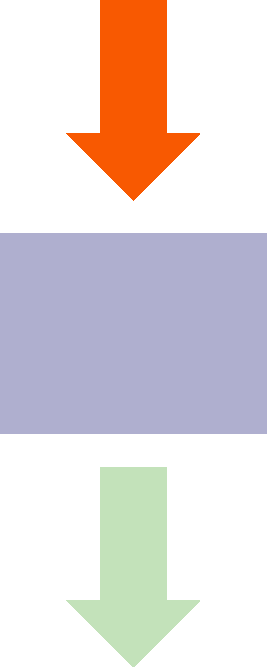
\includegraphics[width=2cm]{img/input}
	\end{column}
\end{columns}
\end{frame}


\begin{frame}
\frametitle{Identificación de Riesgos}
\framesubtitle{Técnicas y Herramientas}

\begin{columns}
	\begin{column}{0.8\textwidth}
\begin{itemize}
    \item<1-> \textbf{Revisiones} de la documentación.
    \item<2-> Técnicas para la \textbf{recopilación} de la información.
    \begin{itemize}
        \item Brainstorming.
        \item Técnica de Delphi.
        \item Entrevistas.
        \item Análisis de las fuentes del problema.
    \end{itemize}
    \item<3-> Análisis con \textbf{listas de chequeo}.
    \item<4-> Análisis de las \textbf{suposiciones}.
    \item<5-> Técnicas de desarrollo de \textbf{diagramas}.
    \begin{itemize}
        \item Diagramas de causa y efecto, flujo del sistema y influencia.
    \end{itemize}
    \item<6-> Análisis SWOT (\textbf{FODA}).
    \item<7-> Juicio de \textbf{Expertos}.
\end{itemize}
	\end{column}
	\begin{column}{0.2\textwidth}
		\includegraphics[width=2cm]{img/tools}
	\end{column}
\end{columns}
\end{frame}

\begin{frame}
\frametitle{Identificación de Riesgos}
\framesubtitle{Valores de Salida}

\begin{columns}
	\begin{column}{0.8\textwidth}
\begin{itemize}
    \item<1-> \textbf{Registro} de riesgos
    \begin{itemize}
        \item<2-> Lista de riesgos \textbf{identificados}.
        \item<3-> Lista de acciones \textbf{potenciales}.
    \end{itemize}
\end{itemize}
	\end{column}
	\begin{column}{0.2\textwidth}
		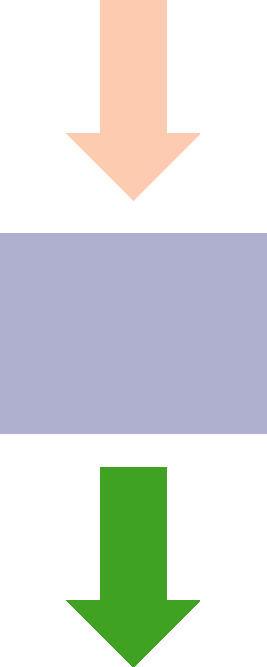
\includegraphics[width=2cm]{img/output}
	\end{column}
\end{columns}
\end{frame}
